% 2011 年陕西卷理科第 16 题：沿高 AD 把 △ABD 折起，使 ∠BDC=90°。左为折前，右为折后。
% 来源 PDF：普通高考/2011/2011陕西理.pdf，SHA-256 04dab6de0e3ee6223a1cbc126f7f83ae354d2b31201a14db1f31c8477d8a3bed。
% 原页：第 1 页第 3 栏下部，书页码 693。
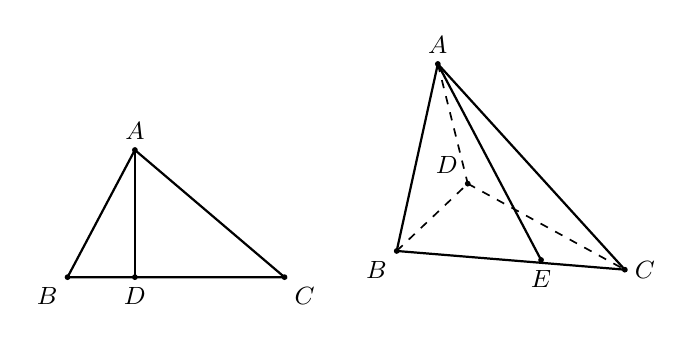
\begin{tikzpicture}[>=stealth, semithick, font=\small, scale=0.95]
  % 折前
  \coordinate (B) at (0,0);
  \coordinate (D) at (0.9,0);
  \coordinate (C) at (2.9,0);
  \coordinate (A) at (0.9,1.7);
  \draw[thick] (B)--(C)--(A)--cycle;
  \draw[thick] (A)--(D);
  \fill (A) circle (1.1pt) node[above] {$A$};
  \fill (B) circle (1.1pt) node[below left] {$B$};
  \fill (C) circle (1.1pt) node[below right] {$C$};
  \fill (D) circle (1.1pt) node[below] {$D$};
  % 折后
  \begin{scope}[xshift=4.4cm]
    \coordinate (B2) at (0,0.35);
    \coordinate (D2) at (0.95,1.25);
    \coordinate (C2) at (3.05,0.1);
    \coordinate (A2) at (0.55,2.85);
    \coordinate (E2) at (1.93,0.23);
    \draw[thick] (A2)--(B2)--(C2)--cycle;
    \draw[thick] (A2)--(E2);
    \draw[dashed] (A2)--(D2) (B2)--(D2) (D2)--(C2);
    \fill (A2) circle (1.1pt) node[above] {$A$};
    \fill (B2) circle (1.1pt) node[below left] {$B$};
    \fill (C2) circle (1.1pt) node[right] {$C$};
    \fill (D2) circle (1.1pt) node[above left] {$D$};
    \fill (E2) circle (1.1pt) node[below] {$E$};
  \end{scope}
\end{tikzpicture}
